\section{Algorithmic Solution}
\label{sec:algorithm}

%As discussed in Section \ref{sec:motivation}, our technique is based on NMF.  
As discussed earlier our technique is based on NMF, and
this particular formulation \eqref{outlier}, which is
suited to outlier analysis, is relatively uncommon, and  does not
have a closed form solution. In order to address this issue we use a
Block Coordinate Descent (BCD) framework and its application to
solve the optimization problem \eqref{outlier}. The BCD framework is
a popular choice not only because of the ease in implementation,
but also because it is scalable. First, we will lay the foundation
for the basic BCD technique, as it generally applies to non-linear
optimization problems. We will then relate it to our non-negative
matrix factorization problem, and explain our algorithm \algofull
(\algo) in detail.

\subsection{Block coordinate Descent}

In this section, we will see relevant foundation for using  this
framework.  Consider a constrained non-linear optimization problem
as follows:
\begin{gather}
\min f(x)\:\mbox{ subject to }\:x \in\mathcal{X},\label{eq:general_nonlinear}
\end{gather}
Here,  $\mathcal{X}$ is a closed convex subset of $\mathbb{R}^{n}$.
An important assumption to be exploited in the BCD method is that
the set $\mathcal{X}$ is represented by a Cartesian product:
\begin{equation}
\mathcal{X}=\mathcal{X}_{1}\times\cdots\times\mathcal{X}_{m},\label{eq:bcd-cartesian-product}
\end{equation}
where $\mathcal{X}_{j}$, $j=1,\cdots,m$, is a closed convex subset
of $\mathbb{R}^{N_{j}}$, satisfying $n=\sum_{j=1}^{m}N_{j}$.
Accordingly, the vector $\mathbf{x}$ is partitioned as
$\mathbf{x}=(\mathbf{x}_{1},\cdots,\mathbf{x}_{m})$ so that
$\mathbf{x}_{j}\in\mathcal{X}_{j}$ for $j=1,\cdots,m$. The BCD
method solves for $\mathbf{x}_{j}$ by fixing all other subvectors of
$\mathbf{x}$ in a cyclic manner. That is, if
$\mathbf{x}^{(i)}=(\mathbf{x}_{1}^{(i)},\cdots,\mathbf{x}_{m}^{(i)})$
is given as the current iterate at the $i^{th}$ step, the algorithm
generates the next iterate
$\mathbf{x}^{(i+1)}=(\mathbf{x}_{1}^{(i+1)},\cdots,\mathbf{x}_{m}^{(i+1)})$
block by block, according to the solution of the following
subproblem:
\begin{equation}
\mathbf{x}_{j}^{(k+1)}\leftarrow\underset{\mathbf{\xi}\in\mathcal{X}_{j}}{\text{argmin}}
f(\mathbf{x}_{1}^{(k+1)},\cdots,\mathbf{x}_{j-1}^{(k+1)},\mathbf{\xi},\mathbf{x}_{j+1}^{(k)},\cdots,\mathbf{x}_{m}^{(k)}).\label{eq:bcd-method}
\end{equation}
Also known as a \textit{non-linear Gauss-Seidel}
method~\cite{Bertsekas1999}, this algorithm updates one block each
time, always using the most recently updated values of other blocks
$\mathbf{x}_{\tilde{j}},\tilde{j}\ne j$. This is important since it
ensures that after each update, the objective function value does
not increase. For a sequence $\left\lbrace
\mathbf{x}^{(i)}\right\rbrace $ where each $\mathbf{x}^{(i)}$ is
generated by the BCD method, the following property holds.
\begin{thm}
\label{thm:bcd}
Suppose $f$ is continuously differentiable in $\mathcal{X}=\mathcal{X}_{1}\times\dots\times\mathcal{X}_{m}$,
where $\mathcal{X}_{j}$, $j=1,\cdots,m$, are closed convex sets.
Furthermore, suppose that for all $j$ and $i$, the minimum of
\[
\min_{\mathbf{\mathbf{\xi}}\in\mathcal{X}_{j}}f(\mathbf{x}_{1}^{(k+1)},\cdots,\mathbf{x}_{j-1}^{(k+1)},\mathbf{\xi},\mathbf{x}_{j+1}^{(k)},\cdots,\mathbf{x}_{m}^{(k)})
\]
is uniquely attained. Let $\left\lbrace
\mathbf{x}^{(i)}\right\rbrace $ be the sequence generated by the
block coordinate descent method as in Eq.~\eqref{eq:bcd-method}.
Then, every limit point of $\left\lbrace
\mathbf{x}^{(i)}\right\rbrace $ is a stationary point. The
uniqueness of the minimum is not required for the case when  $m=2$
\cite{Grippo2000}.
\end{thm}

The proof of this theorem for an arbitrary number of blocks is shown
in Bertsekas~\cite{Bertsekas1999}.
For a non-convex optimization problem, most algorithms only guarantee
the stationarity of a limit point \cite{Lin2007}.

When applying the BCD method to a constrained non-linear programming
problem, it is critical to wisely choose a partition of
$\mathcal{X}$, whose Cartesian product constitutes $\mathcal{X}$. An
important criterion is whether the sub-problems in
Eq.~\eqref{eq:bcd-method} are efficiently solvable. For example, if
the solutions of sub-problems appear in a closed form, each update
can be computed fast. In addition, it is worth checking how the
solutions of sub-problems depend on each other. The BCD method
requires that the most recent values be used for each sub-problem in
Eq.~\eqref{eq:bcd-method}. When the solutions of sub-problems depend
on each other, they have to be computed sequentially to make use of
the most recent values. If solutions for some blocks are independent
of each other,  they can be computed simultaneously. We discuss how
different choices of partitions lead to different NMF algorithms.
The  partitioning can be achieved in several ways, by using either
matrix blocks, vector blocks or scalar blocks.

\subsubsection{BCD with Two Matrix Blocks - ANLS Method}
The most natural partitioning of the variables is to have two big
blocks, $\mathbf{W}$ and $\mathbf{H}$. In this case, following the
BCD method in Eq.~\eqref{eq:bcd-method}, we take turns solving the
following:
%\begin{equation}
%\left\{
%\begin{array}
%\mathbf{W}^{(k+1)}\leftarrow\argmin_{\mathbf{W}\ge0}f(\mathbf{W},\mathbf{H}^{(k)})\\ 
%\mathbf{H}^{(k+1)}\leftarrow\argmin_{\mathbf{H}\ge0}f(\mathbf{W}^{(k+1)},\mathbf{H}).
%\end{array}
%\right.
%\end{equation}

\begin{equation}
\left\{
  \begin{array}{ll}
  \mathbf{W}^{(k+1)}\leftarrow\argmin_{\mathbf{W}\ge0}f(\mathbf{W},\mathbf{H}^{(k)})\\ 
\mathbf{H}^{(k+1)}\leftarrow\argmin_{\mathbf{H}\ge0}f(\mathbf{W}^{(k+1)},\mathbf{H}).  
\end{array}
\right.\label{bcd}
\end{equation}




Since the sub-problems are non-negativity constrained least squares (NLS) problems, the
two-block BCD method has been called the alternating non-negative least
square (ANLS) framework \cite{Lin2007,Kim2008,Kim2011}.

\subsubsection{BCD with 2k Vector Blocks - HALS/RRI Method}
We partition the unknowns into 2k blocks in which each block
is a column/row of $\mathbf{W}$ or $\mathbf{H}$. In this case,
it is easier to consider the objective function in the following
form:
\begin{equation}
f(\mathbf{w}_{1},\cdots,\mathbf{w}_{r},\mathbf{h}_{1}^\intercal,\cdots,\mathbf{h}_{r}^\intercal)=\|\mathbf{A}-\sum_{j=1}^{r}\mathbf{w}_{j}\mathbf{h}_{j}^{T}\|_{F}^{2},\label{eq:nmf_columns_obj}
\end{equation}
where
$\mathbf{W}=[\mathbf{w}_{1},\cdots\mathbf{w}_{r}]\in\mathbb{R}_{+}^{m\times
r}$ and
$\mathbf{H}=[\mathbf{h}_{1},\cdots,\mathbf{h}_{r}]^\intercal\in\mathbb{R}_{+}^{r\times
n}$. The form in Eq.~\eqref{eq:nmf_columns_obj} represents the fact
that  $\mathbf{A}$ can be  approximated by the sum of $r$ rank-one
matrices.

Following the BCD scheme, we can minimize $f$ by iteratively solving
the following:
\[
\mathbf{w}_{i}\leftarrow\argmin_{\mathbf{w}_{i}\ge0}f(\mathbf{w}_{1},\cdots,\mathbf{w}_{r},\mathbf{h}_{1}^\intercal,\cdots,\mathbf{h}_{r}^\intercal)
\]
 for $i=1,\cdots,r$, and
\[
\mathbf{h}_{i}^\intercal\leftarrow\argmin_{\mathbf{h}_{i}^\intercal\ge0}f(\mathbf{w}_{1},\cdots,\mathbf{w}_{r},\mathbf{h}_{1}^\intercal,\cdots,\mathbf{h}_{r}^\intercal)
\]
 for $i=1,\cdots,r$.

% \begin{figure}
% \scalebox{0.42}{\includegraphics{figs/2kblock.eps}}
% \caption{2k-Block Block Coordinate Descent(BCD)}\label{fig:2kblock}
% \end{figure}

The  2K-block BCD algorithm has been studied as Hierarchical
Alternating Least Squares (HALS) proposed by Cichocki et al.
\cite{Cichocki2007,Cichocki2009} and independently by Ho et al.
\cite{Ho2008} as rank-one residue iteration (RRI).

\subsubsection{BCD with k(n + m) Scalar Blocks}
 We can also partition the variables with the smallest  $k(n+m)$ element blocks of scalars, where every element of $\mathbf{W}$ and $\mathbf{H}$ is considered as a block in the context of \ref{thm:bcd}.   To this end, it
helps to write the objective function as a quadratic function of scalar
$w_{ij}$ or $h_{ij}$ assuming all other elements in $\mathbf{W}$
and $\mathbf{H}$ are fixed: \begin{subequations} \label{eq:nmf_element_objective}
\begin{gather}
f(w_{ij})  =  \|(\mathbf{a}_{i}^\intercal-\sum_{\tilde{k}\ne j}w_{i\tilde{k}}\mathbf{q}_{\tilde{k}}^\intercal)-w_{ij}\mathbf{h}_{j}^\intercal\|_{2}^{2}+\mbox{const},\\
f(h_{ij})  =  \|(\mathbf{a}_{j}-\sum_{\tilde{k}\ne i}\mathbf{w}_{\tilde{k}} h_{\tilde{k}j})-\mathbf{w}_{ i}h_{ij}\|_{2}^{2}+\mbox{const},
\end{gather}
\end{subequations} where $\mathbf{a}_{i}^\intercal$ and $\mathbf{a}_{j}$
denote the $i^{th}$ row and the $j^{th}$ column of $\mathbf{A}$,
respectively.

%\begin{figure}
%\scalebox{0.35}{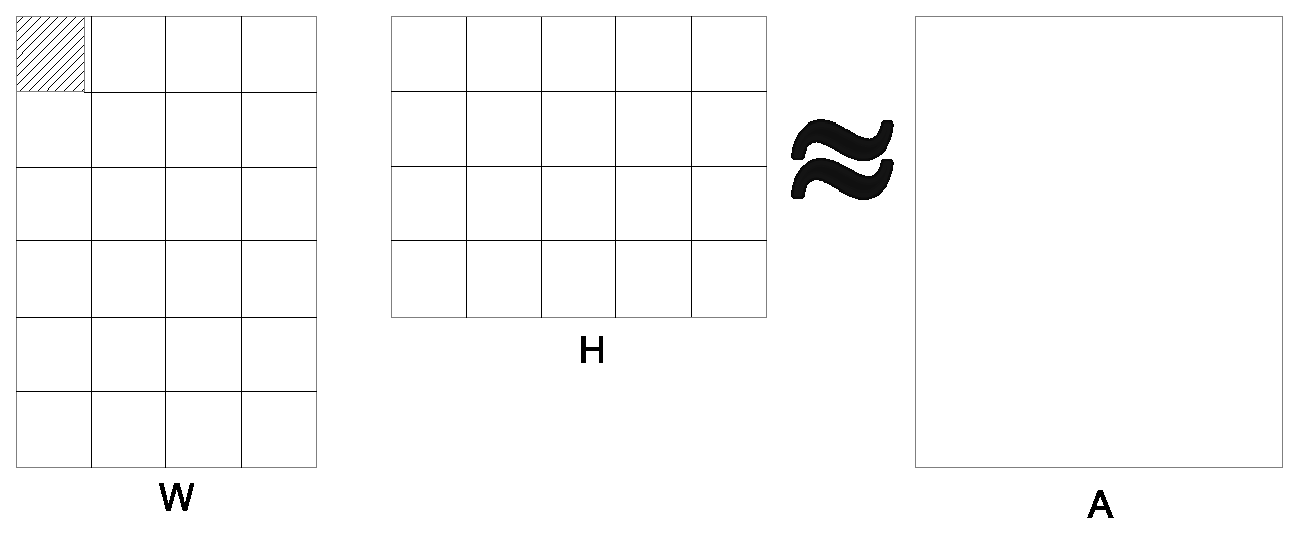
\includegraphics{figs/scalarblock.eps}}
%\caption{Scalar Block BCD}\label{fig:scalarblock}
%\end{figure}

In this paper for solving the optimization problem \eqref{outlier},
we partition the matrices $\mathbf{Z,W,H}$ into vector blocks such
as \linebreak $\mathbf{z_1, \cdots, z_n, w_1, \cdots, w_r, h_1,\cdots, h_r}$. The
reasoning behind this partitioning is explained in the next section.

\subsection{\algofull (\algo)}
In this section, we propose an efficient algorithm for the outlier
detection model \eqref{outlier}.

To determine the $\mathbf{Z,W,H}$ for the aforementioned
optimization problem \eqref{outlier}, we use the  block coordinate
descent method. In other words, by fixing $\mathbf{W,H}$, we
determine the optimal $\mathbf{Z}$ as vector blocks
$\mathbf{z_1,\cdots,z_n}$ and vice versa. Due to $\ell_{1,2}$-norm,
this optimization corresponds to the two block non-smooth BCD
framework.

\begin{equation}
\begin{aligned}
\label{am}
\mathbf{Z}^{(k+1)} & \leftarrow \underset{\mathbf{Z}}{\argmin} \frac{1}{2}\norm{\mathbf{A}-\mathbf{Z}-\mathbf{W}^{(k)}\mathbf{H}^{(k)}}_F^2 \\
                    &\qquad \qquad \qquad \qquad \qquad \qquad \quad     + \alpha \norm{\mathbf{Z}}_{1,2}    \\
(\mathbf{W}^{(k+1)},\mathbf{H}^{(k+1)}) & \leftarrow \underset{\mathbf{W\geq0}, \mathbf{H\geq0}}{\argmin} \frac{1}{2}\norm{\mathbf{A}-\mathbf{WH}-\mathbf{Z}^{(k+1)}}  \\
                                        & \qquad \qquad \qquad \qquad \qquad \qquad \quad + \beta \norm{\mathbf{H}}_1 &    \\
\end{aligned}
\end{equation}
%We have a closed form solution for outlier variable $\mathbf{Z}$. See \ref{thm:updatez}. And, for low rank matrix $\mathbf{W}\mathbf{H}$, we need to solve highly non-convex problems.
Regarding ${\bf Z}=[{\bf z}_1,...,{\bf z}_n]$, the minimization
problem in \eqref{am} has a  separable structure:
$$
\mathbf{Z}^{(k+1)} =  \underset{\mathbf{Z}}{\argmin} \sum_i \frac{1}{2}\norm{\mathbf{\bar{a}}_i -\mathbf{z}_i}_2^2+ \alpha \norm{\mathbf{z}_i}_{2}
$$
where $\mathbf{\bar{a}}_i = {\bf a}_i - ({\bf W}^{(k)}{\bf
H}^{(k)})_i$. Therefore, we only need to define a solution with
respect to one variable ${\bf z}_i$. Thus, we partition the matrix
$\mathbf{Z}$ into vector blocks $\mathbf{z}_i$ and construct
$\mathbf{Z}$ as a set of vectors $\mathbf{z}_i$. Also, the blocks
$\mathbf{z}_i$ is independent of $\mathbf{z}_j, \forall i \neq j$.
That is, the closed form solution of $\mathbf{z}_i$ is dependent
only on $\mathbf{\bar{a}}_i$. When all other blocks of
$\mathbf{w_1,\cdots,w_r,h_1,\cdots,h_r}$, are fixed, every vector
$\mathbf{z}_i \in \mathbf{Z}$, can be solved to optimal in parallel.
Thus, we adhere to BCD framework of solving the vector blocks of
$\mathbf{z}_i$, to optimal, when all the other blocks are fixed.

%Even individually solving, $\mathbf{Z,H}$ are non-convex in the above problem. Hence, let us define a (n+2k) vector block BCD on the above problem.

\begin{thm}\label{thm:updatez}
The solution of the following minimization problem
$$
\mathbf{z}_i^* = \argmin_{\mathbf{z}_i} f({\bf z}_i) = \frac{\gamma}{2}\norm{{\bf z}_i-{\bf a}_i}_2^2 + \alpha \norm{{\bf z}_i}_2
$$
is the generalized shrinkage operator:
$$
{\bf z}_i^* = \mbox{shrink}({\bf a}_i , \frac{\alpha}{\gamma})
$$
where generalized shrinkage operator is defined as:
$$
\mbox{shrink}({\bf a}_i,C) = \mbox{max}(\norm{{\bf a}_i}_2 -C,0)\frac{{\bf a}_i}{\norm{{\bf a}_i}_2}
$$
\end{thm}
\vspace{-0.8in}
\begin{proof}
$$
\frac{\partial f({\bf z}_i)}{\partial {\bf z}_i} = \gamma ({\bf z}_i - {\bf a}_i) + \alpha \frac{{\bf z}_i}{\norm{{\bf z}_i}}
$$
When $\norm{{\bf a}_i}_2 \le \frac{\alpha}{\gamma}$,
$$
f({\bf z}_i) \ge \frac{\gamma}{2}(\norm{{\bf z}_i}^2_2 + \norm{{\bf a}_i}^2_2)  + (\alpha-\gamma\norm{{\bf a}_i}_2)\norm{{\bf z}_i}_2
$$
Therefore we have:
$$
\argmin_{{\bf z}_i} f({\bf z}_i) =0.
$$

When $\norm{{\bf a}_i}_2 \ge \frac{\alpha}{\gamma}$,
let ${\bf z}_i = c{\bf a}_i$ then
$$
\frac{\partial f({\bf z}_i)}{\partial {\bf z}_i} = \gamma ({\bf z}_i - {\bf a}_i) + \alpha \frac{{\bf z}_i}{\norm{{\bf z}_i}_2} = [ \gamma( c - 1 ) + \frac{\alpha}{\norm{{\bf a}_i}}_2 ]{\bf a}_i=0
$$
where
$$
c =  1 - \frac{\alpha}{\gamma}\frac{1}{\norm{{\bf a}_i}_2}.
$$
Therefore, we get
$$
{\bf z}_i =  (\norm{{\bf a}_i}_2 - \frac{\alpha}{\gamma})\frac{{\bf a}_i}{\norm{{\bf a}_i}_2}
$$
Now, utilizing the generalized shrinkage operator as defined in \cite{esser2010}\cite{wang2008},
$$
{\bf z}_i^* = \mbox{shrink}({\bf a}_i,C) = \mbox{max}(\norm{{\bf a}_i}_2 -C,0)\frac{{\bf a}_i}{\norm{{\bf a}_i}_2}
$$
where $C=\alpha/\gamma$.
\end{proof}

%We will find $\mathbf{Z}=(\mathbf{z}_1,\mathbf{z}_2,\cdots,\mathbf{z}_n)$ as separate $n$ vector blocks. Given $\mathbf{A,W,H}$, the optimal value of $\mathbf{z}_i= max(\mathbf{||d||_i}-\alpha,0) \times \frac{\mathbf{d_i}}{||\mathbf{d}_i||}$, where $\mathbf{d}_i$ is the $i$-th column of matrix $\mathbf{D=A-WH}$.
%\begin{proof}
%We will find the $\mathbf{Z}$ as separate $n$ vector blocks. Then, the optimal value of $\mathbf{Z=(z_1,z_2,\cdots z_n)}$ in equation \eqref{bcdoutlier} can be rewritten as
%\begin{equation}
%\begin{aligned}
%\label{bcdupdatez}
%f_\mathbf{z}=\underset{\mathbf{Z}}{argmin}&\sum_{i=1}^n\frac{1}{2}||\mathbf{d}_i-\mathbf{z}_i||^2+\alpha ||\mathbf{z}_i|| \\
%\underline{if \; ||\mathbf{d}_i||_2 > \alpha} \\
%\frac{\partial f_\mathbf{z}}{\partial \mathbf{z}_i}=&
%\mathbf{d}_i-\mathbf{z}_i + \lambda \frac{\mathbf{z}_i}{||\mathbf{z}_i||}   \\
%= & \alpha (\frac{\mathbf{d}_i}{||\mathbf{d}_i||} - \frac{\mathbf{z}_i}{||\mathbf{z}_i||}) \\
%\underline{if \; ||\mathbf{d}_i||_2 < \alpha}\\
%& \frac{1}{2}||\mathbf{d}_i-\mathbf{z}_i||^2+\alpha ||\mathbf{z}_i|| \\
%\geq & \frac{1}{2} ||\mathbf{d}_i|| + \frac{1}{2} ||\mathbf{z}_i|| - ||\mathbf{d}_i|| ||\mathbf{z}_i|| + \alpha ||\mathbf{z}_i|| \\
%\geq & 0 \\
%\end{aligned}
%\end{equation}
%From the above, we can conclude that $\mathbf{z}_i= max(\mathbf{||d||_i}-\alpha,0) \times \frac{\mathbf{d_i}}{||\mathbf{d}_i||}$.
%\end{proof}


%It is interesting to observe here that every $\mathbf{z}_i$ is independent of $\mathbf{z}_j, \forall j \neq i$. Hence the update of $\mathbf{Z}$ can be done in parallel.

Now, we need to solve the following NMF model with sparsity constraints on ${\bf H}$:
$$
({\bf W}^{(k+1)},{\bf H}^{(k+1)}) = \argmin_{{\bf W} \ge 0, {\bf H} \ge 0}  \norm{\bar{\bf A} - {\bf W}{\bf H}}_F^2 + \beta \norm{\bf H}_1
$$
where $\bar{\bf A} = {\bf A} - {\bf Z}^{(k+1)}$. Let
\begin{equation}\label{hals}
{\cal F}({\bf w}_1,...,{\bf w}_r;{\bf h}_1,...,{\bf h}_r) = \norm{\bar{\bf A} - \sum_{i=1}^r {\bf w}_i{\bf h}_i}_F^2 + g({\bf h}_1,...,{\bf h}_r).
\end{equation}
where ${\bf W} = [{\bf w}_1,{\bf w}_2,\dots,{\bf w}_r]$ and ${\bf H} = [{\bf h}_1, {\bf h}_2, \dots, {\bf h}_r]^T$. For any $j \in \{1,...,r\}$, (\ref{hals}) can be rewritten as
\begin{equation}\label{hals-1}
\norm{\bar{{\bf A}}-\sum_{i=1}^r{\bf w}_i{\bf h}_i^T}^2_F=\norm{\bar{\bf A}-\sum_{i=1,i\not=j}^r {\bf w}_i{\bf h}_i^T-{\bf w}_j{\bf h}_j^T}^2_F.
\end{equation}
The following is the framework of the  block coordinate descent
method with a separable regularizer such as the  Frobenius norm. We
iteratively minimize ${\cal F}({\bf W},{\bf H})$ with respect to
each column of ${\bf W}$ and ${\bf H}$ :
\begin{equation}
\left\{
  \begin{array}{ll}
  {\rm for}\ j=1 \dots r \\[5pt]
  {\bf h}_j^{(k+1)} = \underset{{\bf h}_j \ge 0}{\rm argmin} \frac{\alpha}{2}\norm{{\bf w}_j^{(k)}{\bf h}_j^T-(\bar{\bf A}-\tilde{\bf W}^{(k)}_j)}^2_F\\\hspace{3cm} + g({\bf h}_1^{(k+1)},...,{\bf h}_j,...,{\bf h}_r^{(k)}) \\[5pt]
  {\rm end}\\[5pt]
    {\rm for}\ j=1 \dots r \\[5pt]
  \hspace{0.25cm}{\bf w}_j^{(k+1)} = \underset{{\bf w}_j \ge 0}{\rm argmin} \norm{{\bf w}_j ({\bf h}_j^{(k+1)})^T -(\bar{\bf A}-\tilde{\bf H}^{(k+1)}_j)}^2_F \\[5pt]
  {\rm end}\\
\end{array}
\right.\label{halsalter}
\end{equation}
where
$$
\tilde{\bf W}^{(k)}_j = \sum_{i=1}^{j-1}{\bf w}_i^{(k)}({\bf h}_i^{(k+1)})^T + \sum_{i=j+1}^r{\bf w}_i^{(k)}({\bf h}_i^{(k)})^T,
$$
and
$$
\tilde{\bf H}^{(k+1)}_j = \sum_{i=1}^{j-1}{\bf w}_i^{(k+1)}({\bf h}_i^{(k+1)})^T + \sum_{i=j+1}^r{\bf w}_i^{(k)}({\bf h}_i^{(k+1)})^T.
$$

According to \ref{thm:updatez}, the solution of $\mathbf{z}_i$ is independent of
$\mathbf{z}_j, \forall i \neq j $,  and it enables us to solve the
solution in parallel. This is very useful when computing for very
large input matrices. Similarly, the vector blocks of $\mathbf{W, H}$
can also be updated in parallel. Now, we have all the building
blocks for the {\algofull}  algorithm. We will be using
\ref{thm:updatez} and the update for $\mathbf{W,H}$ from
\eqref{halsalter}. The Algorithm \ref{alg:tomf}, gives the outline
of the \algo and its complete implementation can be obtained 
from \url{https://github.com/ramkikannan/outliernmf} to try with
any real world text dataset. 

\begin{algorithm}
  \SetKwInOut{Input}{input}\SetKwInOut{Output}{output}
  \Input{Matrix $\mathbf{A}\in\mathbb{R}_+^{m \times n}$,reduced rank $r$, $\alpha$, $\beta$}
  \Output{Matrix $\mathbf{W}\in\mathbb{R}_+^{m\times r}$,$\mathbf{H}\in\mathbb{R}_+^{r \times n}$,$\mathbf{Z} \in \mathbb{R}^{m \times n}$}
  \BlankLine
    \tcp{Rand initialization of \textbf{W}, \textbf{H}, \textbf{Z}}
    %\tcp{ For other types refer to Section \ref{sec:initialization}}
  \textit{Initialize \textbf{W}, \textbf{H}, \textbf{Z} as a nonnegative random matrix} \;
  \While{stopping criteria $\mathfrak{C}_1$ not met} {
  \tcp{Compute Z for the given $\mathbf{A,W,H},\alpha,\beta$ based on \ref{thm:updatez}} 
  \For{$i \leftarrow 1$ \KwTo $n$}{ \label{alg:loopz}
    $\mathbf{z_i} \leftarrow max(\norm{{\bf a}_i}_2 - \frac{\alpha}{\gamma},0)\frac{{\bf a}_i}{\norm{{\bf a}_i}_2}$
  }
  \While{stopping criteria $\mathfrak{C}_2$ not met}{ \label{alg:innerbcd}
      \For{$j \leftarrow 1$ \KwTo $r$}{
        $ {\bf h}_j^{(k+1)} = \underset{{\bf h}_j \ge 0}{\rm argmin} \frac{\alpha}{2}\norm{{\bf w}_j^{(k)}{\bf h}_j^T-(\bar{\bf A}-\tilde{\bf W}^{(k)}_j)}^2_F+ g({\bf h}_1^{(k+1)},\cdots,{\bf h}_j,\cdots,{\bf h}_r^{(k)})$\;
    }
    \For{$j \leftarrow 1$ \KwTo $r$}{
        ${\bf w}_j^{(k+1)} = \underset{{\bf w}_j \ge 0}{\rm argmin} \norm{{\bf w}_j ({\bf h}_j^{(k+1)})^T -(\bar{\bf A}-\tilde{\bf H}^{(k+1)}_j)}^2_F$\;
    }
  }
}
\caption{\algofull\ (\algo)}\label{alg:tomf}
\end{algorithm}

%\subsection{Implementation Details}
%The entire experimentation for this paper is based on Matlab implementation.
%The implementation challenges of Matlab is different from other low
%languages such as C/C++/Java or frameworks based on low languages.
%In this section, we will describe the challenges that we encountered
%during the implementation of the Algorithm \ref{alg:tomf}.

%One of the challenges is scaling the algorithm. Matlab performs
%poorly on scripts with loops such as {\em for} and {\em while}.
%In our algorithm we have three loops - (1) To find the columns of $\mathbf{Z}$
%in Step \ref{alg:loopz}; (2) Two loops to find  $r$ vectors of $\mathbf{W,H}$ in Step \ref{alg:innerbcd}.
%For practical reasons, generally $r$ is kept low in the order of 100's. However,
%for very large matrices $n$ is in the order of few 100's of thousand's.

%As described earlier, the solution to our problem is embarrassingly parallel.
%Interestingly, all the vectors blocks with in a particular matrix is independent
%of each other. That is, $\mathbf{z}_i \in \mathbf{Z}$
%, \mathbf{w}_i \in \mathbf{W}, \mathbf{h}_i \in \mathbf{H}$
%independent of $\mathbf{z}_j \in \mathbf{Z}, \forall i, i \neq j$ and similarly for
%all the vector blocks of matrix $\mathbf{W,H}$.

%We leveraged this ability of the solution to parallely update the
%vector blocks of one matrix among multiple cores. Now-a-days,
%all the commercial desktop processors such as Intel i7, i5 and i3
%or server processor such as Intel E7 and E5 are by default have
%many cores. The matlab parallel computing toolbox has {\em parfor}
%construct that executes independent blocks parallely among multiple
%cores. Matlab allows simultaneous execution of 12 worker threads parallely
%in a single machine. Using this Matlab feature, we found all the vector
%blocks of every matrix such as $\mathbf{z}_i in \mathbf{Z}$, parallely.
%This reduced the computation time significantly.
%Similar capabilities are also available in other scripting languages
%such as R and python.

% \mathbf{w}_i \in \mathbf{W}, \mathbf{h}_i \in \mathbf{H}$

%The execution of the algorithm is given as part of experimentation section \ref{sec:insights}.

% \begin{corollary}
% Given $\mathbf{A,Z}$, the BCD for solving $\mathbf{W,H}$ based on \eqref{halsalter} in Step \ref{alg:innerbcd} of Algorithm \ref{alg:tomf} converges.
% \end{corollary}
% \begin{proof}
% In this problem we have partitioned of $\mathbf{W,H}$ as vector blocks $\mathbf{w_1,\cdots,w_r,h_1,\cdots,h_r}$. Given other blocks, every time we find an optimal block $\mathbf{h}_j$ of low rank factor $\mathbf{H}$ or the optimal block $\mathbf{w}_j$ of $\mathbf{W}$. According to \ref{thm:bcd}, given $\mathbf{A,Z}$, the BCD for solving $\mathbf{W,H}$ based on \eqref{halsalter} in Step \ref{alg:innerbcd} of Algorithm \ref{alg:tomf} converges.
% \end{proof}

% Similarly, the next theorem discusses about convergence of the Algorithm \ref{alg:tomf}.

% \begin{thm}\label{thm:convergence}
% Given the condition that $\mathbf{W,H}$ are stationary points, the algorithm for finding $\mathbf{Z,W,H}$ also converges.
% \end{thm}
% \begin{proof}
% \woo{complete this proof.}
% \end{proof}
